\documentclass{article}
\usepackage[utf8]{inputenc}
\usepackage{mathtools}
\usepackage{enumerate}
\usepackage{pgfplots}
\usepackage{tikz}
\usepackage{amsthm}
\usepackage{amssymb}
\usepackage{float}
\usepackage{anysize}

\marginsize{2cm}{2cm}{2cm}{2cm}

\title{Sistemas expertos probabilísticos}
\author{Anabel Gómez Ríos\\
        Jacinto Carrasco Castillo}
\date{Mayo 2016}

% Definición de estilo de definición
\newtheoremstyle{definition_wo_parentheses}
  {\topsep}% measure of space to leave above the theorem. E.g.: 3pt
  {\topsep}% measure of space to leave below the theorem. E.g.: 3pt
  {}% name of font to use in the body of the theorem
  {0pt}% measure of space to indent
  {\bfseries}% name of head font
  {.}% punctuation between head and body
  { }% space after theorem head; " " = normal interword space
  {\thmname{#1}\thmnumber{ #2.}\thmnote{ #3}}
  
  
\theoremstyle{definition_wo_parentheses}	
\newtheorem{definicion}{Definición}

\begin{document}

\maketitle

\section{Introducción}
En clase hemos visto sistemas expertos basados en reglas del tipo \textbf{SI} \textit{condición} \textbf{ENTONCES} \textit{acción} (donde tanto en \textit{condición} como en \textit{acción} pueden aparecer expresiones lógicas compuestas). En estos sistemas se comprueba si \textit{condición} es cierta o no y, en caso de serlo, se lleva a cabo \textit{acción}.\\

Este tipo de sistemas son muy útiles y muy utilizados por su simplicidad y el parecido con el razonamiento humano, pero presentan varios inconvenientes:
\begin{enumerate}
    \item Mantener la coherencia entre las reglas de la base de conocimiento. Pueden aparecer dos tipos de problemas: encadenamientos infinitos, cuando aparecen reglas del tipo \textit{Si A entonces B} junto con \textit{Si B entonces A} y problemas de ampliación en la base de conocimiento cuando hay que realizar una actualización y para mantener la coherencia la base de datos se hace innecesariamente grande, llegando incluso a ser mejor reconstruirla de nuevo.
    \item Dificultades para retractarse de anteriores conclusiones debido al carácter modular y monótono de estos sistemas, ya que cuando se cumple la condición de una regla, se da la acción sin tener en cuenta el resto del conocimiento.
    \item Opacidad: Al tener que dividir el conocimiento en pequeñas reglas, se pierde perspectiva global del problema tratado.
    \item Ineficiencia provocada por la continua comprobación de las reglas en cada iteración.
\end{enumerate}

Sin embargo el principal problema es que cuando se trabaja con problemas reales y conocimiento humano en la mayoría de los casos hay inherente incertidumbre bien en los hechos (en el conocimiento, que no se conoce completamente), o bien en las reglas que son incompletas, imprecisas o inconsistentes.\\
Normalmente, las evidencias que tenemos sobre un hecho no nos permiten deducir con seguridad las conclusiones o la negación de las mismas, pero sí nos permiten dar mayor credibilidad a una regla.

\section{Ejemplo de sistema experto Probabilístico: MYCIN}
MYCIN fue el primer sistema experto que consideró conocimiento incierto. En este sistema, una regla \textbf{Si} A \textbf{Entonces} B se representaba $A \overset{m}{\rightarrow}B$, expresando que si se conoce $A$, entonces se puede actualizar la certeza de $B$ en cierta cantidad, en función de la fuerza de la regla, $m$. El valor $m$ se denomina factor de certeza de la regla y toma valores en el intervalo $[-1,1]$.\\

Supongamos el siguiente ejemplo:
\[A \overset{m_1=0.8}{\longrightarrow} B ; B\ y\ C \overset{m_2=0.7}{\longrightarrow} D
\]
y observamos $A$ (y por tanto la certeza de $A$, que vamos a representar $Ctz(A)$ es 1) y la certeza sobre $C$ es 0.6. Entonces, nuestra creencia de $B$ se actualiza a un valor 0.8, $Ctz(B)=0.8$ y tenemos que actualizar la certeza sobre $D$. En estos casos, MYCIN calcula el valor de certeza para la sentencia $B\ y \ C$ como una función de las certezas de $A$ y $B$: $Ctz(B\ y\ C) = min{0.8,0.6}=0.6$ y por tanto $Ctz(D)=0.6*0.7=0.42$.\\

Después comentaremos mecanismos de propagación que permiten trabajar con sistemas más complejos.

\section{Comparación con los sistemas expertos basados en reglas}

\subsection{Base de conocimiento}

El conocimiento de un sistema experto basado en reglas consiste en los hechos y el conjunto de reglas. En un sistema experto basado en probabilidad, el conocimiento viene dado por un espacio de probabilidad que incluye las variables, sus posibles valores y su función de probabilidad conjunta. En ambos sistemas los datos consisten en la evidencia asociada a los casos a analizar.\\
Las diferencias también se encuentran en la dificultad para implementar la base de conocimientos. Mientras que en el sistema experto basado en reglas ``sólo'' necesitamos usar elementos como objetos, conjunto de valores, premisas, conclusiones y reglas; en los sistemas expertos basados en probabilidad el conocimiento puede ser mucho más extenso. Por contra, son necesarios numerosos parámetros, lo que dificulta su definición.

\subsection{Motor de inferencia}

El motor de inferencia también es más sencillo de implementar en los sistemas expertos basados en reglas, ya que obtenemos las conclusiones a partir de los hechos aplicando estrategias de inferencia como \textit{modus ponens}, \textit{modus tollens} y encadenamiento de reglas. En los sistemas expertos basados en probabilidad, el motor de inferencia se basa en la evaluación de las probabilidades condicionales, utilizando uno o varios métodos propuestos por diferentes tipos de sistemas expertos probabilísticos. El grado de dificultad de implementar un motor de inferencia probabilístico será mayor y crece si usamos modelos de dependencia generales en detrimento de modelos de independencia.

\subsection{Subsistema de explicación}

La explicación en el sistema basado en reglas viene dada por las reglas que se han activado para determinar esa conclusión en cada momento. En el caso probabilístico la información sobre qué variables influyen en otras está codificada en la función de probabilidad conjunta, lo que hace que la explicación se base en los valores relativos de las probabilidades condicionales que miden los grados de dependencia. Una comparación de las probabilidades condicionales para diferentes conjuntos de evidencia permite analizar sus efectos en las conclusiones.

\subsection{Subsistema de aprendizaje}

En los sistemas expertos basados en reglas, el aprendizaje consiste en incorporar nuevos objetos, valores factibles para los objetos, nuevas reglas o modificaciones de los conjuntos existentes, valores posibles o reglas. En los sistemas expertos probabilísticos, consiste en incorporar o modificar la estructura del espacio de probabilidad: variables, posibles valores o parámetros.

\section{Teoría de la Probabilidad}
Vamos a ver algunas nociones básicas de probabilidad que serán de utilidad para trabajar con este tipo de sistemas.

\subsection{Probabilidad marginal}
Sean $X_1,X_2,...,X_n$ un conjunto de variables aleatorias que toman valores discretos y sea $\{x_1,x_2,...,x_n\}$ el conjunto de los posibles valores que pueden tomar. Sea $P(x_1,x_2,...,x_n)$ una probabilidad sobre $X_1,X_2,...,X_n$, es decir, $P(x_1,x_2,...,x_n) = P(X_1 = x_1,...,X_n=x_n)$, entonces la distribución de probabilidad marginal sobre la $i$-ésima variable se obtiene mediante
\[	P(x_i) = P(X_i=x_i) = \sum_{x_1,...,x_{i-1},x_{i+1},...,x_n}P(x_1,...,x_n)	\]

\subsection{Probabilidad condicionada}
Sean $X$ e $Y$ dos conjuntos disjuntos de variables que toman valores en $\{x_1,...,x_n\}$ y $\{y_1,...,y_m\}$. La distribución de probabilidad condicionada de $X$ dado que $Y=y_j$ (con $j \in \{1,...,m\}$ y $P(Y=y_j)>0$) viene dada por
\[	\forall x_i \in X;\ P(X=x_i|Y=y_j)=P(x_i|y_j)=\frac{P(x_i,y_j)}{P(y_j)}	\]
Por tanto, la distribución de probabilidad conjunta puede obtenerse como:
\[	P(x_i,y_j)=P(y_j)P(x_i|y_j)	\]
La distribución de probabilidad conjunta nos va a permitir actualizar nuestro conocimiento a la luz de nueva información.

\subsection{Independencia probabilística}
Sean $X$ e $Y$ dos subconjuntos disjuntos del conjunto de variables aleatorias $\{X_1,...,X_n\}$. Se dice que $X$ es \textbf{marginalmente independiente} de $X$ y se nota $I(X,\emptyset,Y)$, si y solamente si para todos los posibles valores $x$ de $X$ e $y$ de $Y$ se satisface que $P(x|y)=P(x)$.\\
En caso contrario, se dice que $X$ es marginalmente dependiente de $Y$, y se denota $\neg I(X,\emptyset,Y)$.\\

Sean $X, Y$ y $Z$ tres conjuntos disjuntos de variables. Se dice que $X$ es \textbf{condicionalmente independiente} de $Y$ dado que conocemos $Z$, y lo notamos $I(X,Z,Y)$, si y sólo si para todos los valores $x,y,z$ de $X,Y,Z$ (respectivamente) se satisface que $P(x|z,y)=P(x|z)$.\\
En caso contrario se dice que son condicionalmente dependientes, y lo notamos por $\neg I(X,Z,Y)$.

\subsection{Teorema de Bayes}
Este teorema nos permite representar la probabilidad condicionada $P(y|x)$ mediante la expresión:
\[	P(y|x)=\frac{P(x|y)P(y)}{P(x)}	\]
Si tenemos en cuenta que $P(x) = \sum_{y \in Y}P(x,y)$ y que $P(x,y) = P(x|y)P(y)$ podemos reescribir la anterior expresión:
\[	P(y|x) = \frac{P(x|y)P(y)}{\sum_{y \in Y} P(x|y)P(y)}	\]

\section{Sistemas Expertos Probabilísticos}
Como hemos dicho, en un sistema experto probabilístico la base de conocimiento está formada por un conjunto de variables $X_1,...,X_n$ y una distribución de probabilidad conjunta sobre ellas $P(x_1,...,x_n)$ y el motor de inferencia es el cálculo de la probabilidad condicional $P(X|E)$.\\
Si tratamos de realizar una aproximación directa, en la que representamos la distribución de probabilidad conjunta con una tabla, nos daremos cuenta de que, incluso en problemas con un conjunto pequeño de variables, el problema es intratable. Sin embargo, son muchas las aplicaciones prácticas en las que se conoce \textit{a priori} que, por ejemplo, dos variables son (marginal o condicionalmente) independientes. En estos casos, podemos utilizar dicha información para hacer el problema tratable. La idea es dividir la distribución conjunta en un conjunto de distribuciones más pequeñas que tengan la misma representatividad, siendo necesario después proporcionar un método que permita recuperar los valores originales de la distribución de probabilidad conjunta.\\
La idea básica es codificar el conocimiento de tal forma en la misma representación no sea necesario el utilizar información que sea irrelevante y la información relevante sea fácilmente accesible. Dos de estos modelos son las redes de Markov y las redes Bayesianas. Ambos sistemas se apoyan en modelos gráficos para representar de forma explícita las relaciones de dependencia e independencia entre las variables.

\section{Redes de Markov}
Las redes de Markov se representan gráficamente mediante grafos no dirigidos, donde los nodos representan las variables y una relación de dependencia entre dos variables se representa mediante la existencia de un camino o conexión entre ellas. Por otra parte, en estos modelos también se representan las relaciones de independencia. En concreto, si $X,Y$ y $Z$ son conjuntos disjuntos de variables, entonces:
\begin{enumerate}
\item Una independencia marginal viene representada por la inexistencia de conexión entre las variables de $X$ e $Y$.
\item Una relación de independencia condicionada del tipo $I(X,Z,Y)$ se representa por el hecho de que todo camino que conecta las variables de $X$ con variables de $Y$ contiene algún nodo de $Z$. Por tanto, si los nodos en $Z$ son borrados del grafo, las variables $X$ e $Y$ quedan desconectadas.
\end{enumerate}

De esta forma, somos capaces de determinar cuándo dos variables son dependientes o no. Pero, ¿puede el modelo gráfico representar todas las relaciones de dependencia / independencia que se derivan de una distribución de probabilidad conjunta?\\
La respuesta a esta pregunta es que no. Supongamos el siguiente ejemplo:

\begin{figure}[H]
\centering
\includegraphics[width=0.3\textwidth]{ejemplo}
\caption{Ejemplo} \label{fig:ejemplo}
\end{figure}

De aquí podemos deducir varias cosas:
\begin{enumerate}
\item Como $P(x|y)=\frac{P(x,y)}{P(y)} = \frac{0.245+0.105}{0.03+0.12+0.245+0.105} = \frac{0.35}{0.5} = 0.7$ y $P(x)=0.21+0.14+0.245+0.105 = 0.7$ tenemos que $P(x|y)=P(x)$ y por tanto $X$ es independiente marginalmente a $Y \Rightarrow$ no existe un camino que conecte $X$ con $Y$.
\item De forma análoga se puede comprobar que $P(x|z)\neq P(x)$ y por tanto existe un camino que conecta $X$ y $Z$ e igualmente con $Z$ e $Y$.
\end{enumerate}

Nos queda por tanto el siguiente grafo:
\begin{center}
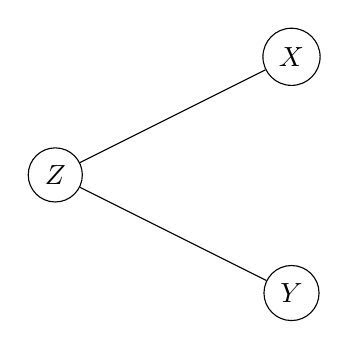
\begin{tikzpicture}[y=.3cm, x=.3cm,font=\normalsize]

\node[draw, circle] (X) at (10,10) {$X$};
\node[draw, circle] (Y) at (10,0) {$Y$};
\node[draw, circle] (Z) at (0,5) {$Z$};

\draw (X) -- (Z);
\draw (Z) -- (Y);

\end{tikzpicture}
\end{center}

De aquí podemos deducir que existe un camino que conecta $X$ con $Y$, el que pasa por $Z$, en contra de la primera deducción. Las redes de Markov por tanto no son capaces de representar relaciones de independencia no transitivas. Una herramienta para diseñar sistemas expertos probabilísticos utilizando el formalismo más potente de los grafos dirigidos para representar las relaciones entre las variables son las redes bayesianas, que veremos a continuación.

\section{Redes bayesianas}

\subsection{Conceptos previos}

Las redes bayesianas son uno de los modelos con más importancia en los sistemas expertos probabilísticos. Gráficamente consisten en un grafo dirigido acíclico, donde los nodos son variables del problema a resolver. Las redes bayesianas permiten representar dos aspectos del conocimiento:

\begin{enumerate}
\item \textbf{Cualitativo}: Relaciones de dependencia e independencia entre variables. Dos variables conectadas por un arco estarán relacionadas.
\item \textbf{Cuantitativo}: Fuerza con la que nos creemos las relaciones de relevancia o dependencia.
\end{enumerate}

Usaremos la representación mediante grafos para indicar la dependencia, por ejemplo, suponemos que representamos un problema que trata del alquiler de un vehículo para un viaje. Las variables son el \textit{Tipo de Vehículo}, \textit{Tipo de Carretera}, \textit{Velocidad Media} durante el viaje, \textit{Duración}, \textit{Precio} del alquiler y \textit{Kilómetros} a recorrer. Si hay un arco, habrá dependencia. 

\begin{center}
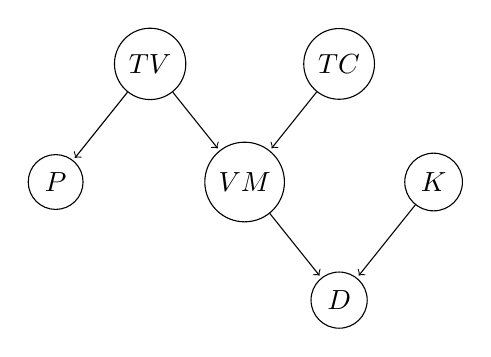
\begin{tikzpicture}[y=.3cm, x=.3cm,font=\normalsize,shorten >=1pt,->]

\node[draw, circle] (P) at (0,5) {$P$};
\node[draw, circle] (TV) at (4,10) {$TV$};
\node[draw, circle] (VM) at (8,5) {$VM$};
\node[draw, circle] (TC) at (12,10) {$TC$};
\node[draw, circle] (D) at (12,0) {$D$};
\node[draw, circle] (K) at (16,5) {$K$};

\draw (TV) -> (P);
\draw (TV) -> (VM);
\draw (VM) -> (D);
\draw (TC) -> (VM);
\draw (K) -> (D);

\end{tikzpicture}
\end{center}

Podemos decir que \textit{TC} y \textit{D} son variables dependientes, en cambio si conocemos \textit{VM} (velocidad media del viaje, \textit{TC} y \textit{D} son independientes. Esto induce el concepto de \textit{d-separación}.

\begin{definicion}[d-separación]
	Si $X,Y,Z$ son subconjuntos disjuntos de nodos en $G$ GDA (grafo dirigido acíclico), entonces $Z$ \textbf{d-separa} $X$ de $Y$ ($<X|Z|Y>_G$) si todos los caminos entre cualquier nodo de $X$ y cualquier nodo de $Y$ están bloqueados por $Z$. 
\end{definicion}

Esto nos permite representar las relaciones entre las variables. Ahora veremos cómo expresarlo de forma numérica. Supongamos dadas dos variables $X,Y$, $X \rightarrow Y$, debido a que hay una dependencia entre las dos variables. La incertidumbre asociada a este tipo de relaciones la podemos representar mediante el uso de una distribución de probabilidad condicionada sobre $Y$ dado $X$, $P(Y|X)$.\\
Cuando tenemos los valores para las distribuciones de probabilidad condicionadas, construimos la distribución de probabilidad conjunta sobre $X_1, \dots, X_n$:
\[ P(X_1, \dots,X_n) = \prod\limits_{i=1}^n P(X_i,\Pi(X_i))\]

donde $\Pi(X_i)$ representa el conjunto de padres de un nodo $X_i$ en la red.\\

Si relacionamos esto con el concepto de d-separabilidad visto anteriormente tenemos:

\begin{equation}
	<X|\emptyset|Y>_G \rightarrow P(X,Y) = P(X) P(Y)
\end{equation}
\begin{equation}
	<X|Y|Z>_G \rightarrow P(X|Y) = P(X|Y,Z)
\end{equation}

\subsection{Redes bayesianas y modelos de dependencia}

Para considerar un GDA, al que hemos asociado un conjunto de distribuciones de probabilidad para cada nodo, como una representación de una distribución de probabilidad conjunta es necesario que ciertas relaciones de independencia del grafo sean válidas en la distribución de probabilidad. En cambio dada una distribución de probabilidad no siempre es posible construir el grafo.

\begin{definicion}[Red bayesiana]
Una red bayesiana es un par $(G(X,A),P)$ donde $G$ es GDA, $X$ es el conjunto de vértices (variables), $A$ el conjunto de arcos y $P=\{P(X_1|\Pi_1),\dots,P(X_n|\Pi_n)\}$ es un conjunto de $n$ funciones de probabilidad condicionada, una para cada variable, y $\Pi_i$ es el conjunto de padres de $X_i$ en $G$. El conjunto $P$ define una función de probabilidad asociada mediante la factorización
\[ P(X) = \prod\limits_{i=1}^n P(X_i|\Pi_i)	\]
\end{definicion}

Toda relación de independencia de la red es una relación de independencia válida en la distribución de probabilidad $P(X)$.Esto permite detectar cuándo la información que proporciona una determinada variable es relevante ante una determinada consulta.

\subsection{Construcción del sistema experto probabilístico}

La base de conocimiento de un sistema experto probabilístico está formada por un conjunto de variables y una distribución de probabilidad conjunta sobre ellas. Para especificar la base de conocimientos se suele hacer uso de modelos más sofisticados que factoricen la distribución en funciones de tamaño menor. Los pasos para el diseño del sistema experto son:

\begin{itemize}
\item \textbf{Planteamiento del problema}. Es fundamental tener una buena definición del problema para mejorar los resultados obtenidos.
\item \textbf{Selección de variables}. Después se selecciona el conjunto de variables relevantes.
\item \textbf{Adquisición de la información cualitativa}. Si disponemos de un experto le pediremos que muestre las relaciones relevantes (también las de independencia). Es de utilidad basarse en modelos gráficos.
\item \textbf{Adquisición de la información cuantitativa}. Este último paso consiste en asignarle valores a la distribución de probabilidad conjunta que tenemos que almacenar en cada nodo en la red. Es conveniente que el experto pueda colaborar con especialistas en estadística para mejorar la calidad de los datos y validar.
\end{itemize}


\section{Métodos de propagación}
Vamos a ver ahora cómo propagar el impacto de una nueva evidencia a través de una Red Bayesiana de manera que las nuevas asignaciones de certidumbre sobre las variables del modelo sean consistentes con los axiomas de la probabilidad.\\
El mecanismo para obtener conclusiones a partir de la evidencia se conoce como propagación de evidencia. Existen tres tipos distintos de algoritmos de propagación: exactos, aproximados y simbólicos. Los exactos son aquellos que calculan las probabilidades de los nodos sin otro error que el resultante del redondeo producido por las limitaciones del cálculo del ordenador. Los aproximados son los que utilizan distintas técnicas de simulación para obtener valores aproximados de las probabilidades y se utilizan en los casos en los que los algoritmos exactos no son aplicables o son computacionalmente costosos. Los algoritmos de propagación simbólica son aquellos que pueden operar no sólo con parámetros numéricos, sino también con parámetros simbólicos, obteniendo las probabilidades en forma simbólica, es decir, en función de los parámetros.\\

Aquí vamos a dar la idea de algunos de estos métodos, pero cabe destacar que hay muchos más, y que si se desea ver el procedimiento completo, se puede ver en la referencia [1].

\subsection{Métodos Exactos}

\subsubsection{Propagación de evidencia}
La propagación de evidencia es una de las tareas más importantes del sistema experto, ya que permite obtener conclusiones cuando se dispone de nueva información. Supóngase un conjunto de variables discretas $X=(X_1,...,X_n)$ y una función de probabilidad $P(x)$, en $X$. Cuando no se dispone de ninguna información, es decir, cuando no existe evidencia, el proceso de propagación consiste en calcular las probabilidades marginales $P(X_i=x_i)$ para cada $X_i \in X$. Estas probabilidades proporcionan información "a priori" sobre los distintos valores que pueden tomar las variables.\\
Cuando se dispone de cierta evidencia, es decir, de un conjunto de variables $E \subset X$ que tienen asociadas los valores $X_i = e_i$ para $X_i \in E$, el proceso de propagación debe tener en cuenta estos valores para calcular las nuevas probabilidades de los nodos. De esta forma, la propagación de evidencia consiste en calcular las funciones de probabilidad condicionada $P(x_i|e)$ para cada variable $X_i$ dada la evidencia $E=e$.\\

El problema de este método es el elevado número de combinaciones de valores que involucra, lo que lo hace altamente ineficiente, incluso en redes con un número reducido de variables.

\subsubsection{Propagación en poliárboles}
La característica principal de este algoritmo es que su complejidad es lineal en el tamaño de la red (número de nodos y aristas de la misma), a diferencia del método anterior.\\
El poliárbol es uno de los modelos gráficos más simples para construir redes bayesianas. Son árboles en los que los nodos pueden tener más de un padre. Además cumplen la propiedad de que dos nodos cualesquiera están unidos por un único camino, lo que implica que cada nodo del poliárbol divide al mismo en dos poliárboles inconexos, uno conteniendo a los padres del nodo por el que dividimos y otro conteniendo a los hijos.\\
En este tipo de grafos, el proceso de propagación puede realizarse como hemos dicho, de modo eficiente combinando la información procedente de los distintos subgrafos mediante el envío de mensajes (cálculos locales) de un subgrafo a otro. Supóngase que se conoce una cierta evidencia $E=e$ y que se quieren calcular las probabilidades $p(x_i|e)$ para todos los valores $x_i$ de un nodo cualquiera $X_i$ que no esté contenido en $E$. Para facilitar el cálculo de estas probabilidades, el conjunto de evidencia $E$ se puede descomponer en dos subconjuntos disjuntos, cada uno de los cuales está contenido en uno de los poliárboles separados por el nodo $X_i$ en el poliárbol original. Por tanto, $E$ se puede descomponer como:
\begin{enumerate}
\item $E_i^+$, que es el subconjunto de $E$ accesible desde $X_i$ a través de sus padres.
\item $E_i^-$, que es el subconjunto de $E$ accesible desde $X_i$ a través de sus hijos.
\end{enumerate}
Por tanto, se tiene $E=E_i^+ \cup E_i^-$. La idea es que a su vez, $E_i^+$ y $E_i^-$ se pueden descomponer en $p$ y $p'$ subconjuntos disjuntos, uno por cada padre en cada subconjunto, y utilizando la independencia de los subconjuntos, se puede ver que un nodo $X_i$ puede calcular su evidencia una vez haya recibido los mensajes de todos sus padres (e igualmente con los hijos)

\subsubsection{¿Qué ocurre cuando hay ciclos?}
Como hemos comentado, el método anterior sólo sirve cuando no hay ciclos, puesto que los padres de un nodo pueden compartir información (es decir, cada padre no puede influir independientemente de los demás sobre la probabilidad de sus hijos comunes).\\
Hay una serie de métodos que pueden usarse cuando se presentan ciclos, como el método de condicionamiento y el método de agrupamiento. La idea fundamental del primero es cortar los múltiples caminos entre los nodos mediante la asignación de valores a un conjunto reducido de variables contenidas en los bucles, obteniendo un poliárbol en el se puede aplicar el método anterior. El segundo método construye representaciones auxiliares de estructura más simple, uniendo conjuntos de nodos del grafo original, hasta que se obtiene de nuevo un poliárbol.

\subsection{Métodos de propagación aproximada}

La idea básica de estos métodos consiste en generar una muestra de tamaño $N$ a partir de la función de probabilidad conjunta de las variables, y luego utilizar la muestra generada para calcular valores aproximados de las probabilidades de ciertos sucesos dada la evidencia. Se pueden separar en dos tipos, los métodos de simulación estocástica, que generan la muestra a partir de la función de probabilidad conjunta usando algunos mecanismos aleatorios, y los métodos de búsqueda determinista, que generan la muestra de forma sistemática.

\subsection{Métodos de propagación simbólica}

Los métodos anteriores requieren que la función de probabilidad conjunta del modelo se especifique numéricamente, es decir, que se asignen valores a todos los parámetros. Esto puede no ser posible, y es en estos casos en los que se utilizan los métodos de propagación simbólica. Estos métodos conducen a soluciones que se expresan como funciones de los parámetros. Por ello, las respuestas a cuestiones generales pueden darse en forma simbólica en función de los parámetros, y las respuestas a preguntas específicas pueden obtenerse sin más que sustituir los valores de los parámetros en la solución simbólica, sin necesidad de rehacer la propagación.

\section{Bibliografía}

\begin{enumerate}
\item \textit{Sistemas expertos y modelos de redes probabilísticas}, Enrique Castillo, José Manuel Gutiérrez y Ali S. Hadi.
\item \textit{Sistemas expertos probabilísticos}, Gámez Martín y Puerta Callejón, disponible en Google Books.
\end{enumerate}


\end{document}